% !TEX root = ../../main.tex
% !TeX spellcheck = de_DE

\chapter{Stand der Technik}
In diesem Kapitel soll ein grundlegendes Verständnis für die genutzten Technologien vermittelt werden.
Außerdem wird erläutert, weshalb die gewählten Frameworks und Techniken für diese Arbeit am geeignetsten sind.

\section{Neuronale Netze}
\todo{Quelle \cite{hyperparameters-search}}

\todo[inline, shadow]{bild von wikipedia ok?}
\begin{figure}[H]
	\centering
	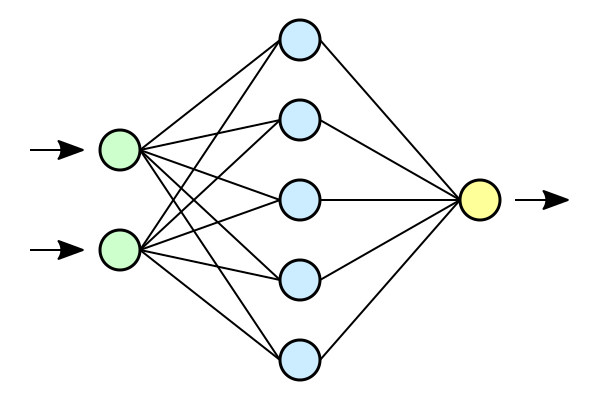
\includegraphics[width=8cm]{kapitel/2_stand_der_technik/img/neural_networks.png}
	\label{img:neural-networks}
	\caption{Neuronales Netz \cite{img:neural-networks}}
\end{figure}

Künstliche Neuronale Netze stellen ein Teilgebiet des Bereichs Künstliche Intelligenz dar.
Durch sie können komplexe Aufgaben, wie Gesichtserkennung, Erkennung von Betrugsfällen oder die Generierung von Bildern mit Computerprogrammen gelöst werden.
\newline

Neuronale Netze bestehen aus synthetischen Neuronen, wobei sich beides am jeweiligen biologischen Vorbild orientiert.
In der Grafik \cref{img:neural-networks} sind die Neuronen als farbige Kreise gekennzeichnet.
Die Aufgabe eines Neurons besteht in der Umwandlung eines oder mehrere Eingangssignale in eine Ausgangssignal.
Für die Umwandlung wird die Summe aller Eingaben berechnet und auf eine Activation-Function angewendet.
Der resultierende Wert wird an alle Ausgaben weitergegeben.
Der Prozess wird durch die folgende Formel mit der Aktivierungsfunktion $\varphi$ verdeutlicht:
\[ Ausgabe = \varphi ( \sum_{n=0}^N Eingabe[n] )\]

Neuronen sind in der Regel in Schichten sortiert, die jeweils mit der vorherigen Schicht verbunden sind.
Damit die Neuronen der verschiedenen Schichten miteinander kommunizieren können, gibt es Übergänge, die in \cref{img:neural-networks} als schwarze Linien dargestellt sind.
Jeder Übergang besitzt einen Weight, das mit dem zu übertragenden Wert multipliziert wird.
Dadurch wird die Komplexität des Modells erhöht, wodurch komplexere Aufgaben gelöst werden können.
\newline

Neuronale Netze werden nicht im klassischen Sinne programmiert, sondern stattdessen definierte Netzarchitekturen trainiert.
Der Trainingsprozess orientiert sich dabei wieder an natürlichen Lernvorgängen.
Dabei gibt es verschiedene Herangehensweisen wie unter anderem Supervised oder Unsupervised Learning.
Bei ersterem existiert im Gegensatz zu letzterem eine vorgegebene Lösung für jede Eingabe.
Beide Verfahren, und nicht an dieser Stelle genannte, haben Vor- und Nachteile, ihre Anwendung ergibt sich meistens aus den vorhanden Daten und gewünschten Ergebnissen.
Darauf soll aber nicht weiter eingegangen werden.
Ziel des Trainings ist die Anpassung der Weights der Übergänge zwischen den Neuronen.
Sie werden im Kontext des Trainingsprozesses auch Parameter genannt.
Durch die Anpassung der Parameter passt sich das Netz den Daten an und erlaubt so verschiedenste Aufgaben zu lösen.
\newline

Für das Training müssen zusätzliche Konfigurationen festgelegt werden, die Hyperparameter genannt werden.
Im Gegensatz zu den Parametern neuronaler Netze werden sie durch das Training nicht verändert.
Bei Hyperparametern handelt es sich zum Beispiel um die Lernrate oder Lossfunction \cite{hyperparameters-gan-using-genetic-algorithm}.
Die Bestimmung von Hyperparametern ist wichtig für den Trainingserfolg des Modells und sollte für jeden Datensatz neu bestimmt werden.
Es sind auch nicht alle Hyperparameter gleichbedeutend für den Trainingserfolg, beispielsweise die Lernrate zählt zu den dominanteren Faktoren \cite{learning-rate-most-important}.
Die Suche nach optimalen Hyperparametern ist sehr komplex, weswegen spezielle Suchverfahren entwickelt wurden. \todo{Überleitung zu Hyperparam Suchverfahren?}

\section{DeepLearning Framework}
Die Implementierung von DeepLearning-Algorithmen ist im Bereich der Künstlichen Intelligenzen eine bedeutende Thematik.
Vor allem die effiziente Ausnutzungen gegebener Hardware stellt eine enorme Herausforderung dar. 
Deshalb existieren über verschiedene Abstraktions-Level diverse Frameworks und Bibliotheken, welche die Arbeit deutlich erleichtern.
\newline

Aufgrund der hohen Rechenkern-Anzahl und der daraus resultierende Multithreading-Charakteristik, eignen sich Grafikkarten besonders gut für DeepLearning-Berechnungen \cite{gpu-for-dl}.
Grafikarten Hersteller stellen dafür Low-Level-APIs bereit, in der Routinen wie Matrix-Multiplikationen oder Aktivierungs-Funktionen hardware-beschleunigt werden.
Dabei kann in den Zugang zu allgemeinen GPU-Operationen (API-Beispiel: CUDA) oder speziellen Funktionen für DeepLearning und Neuronale Netze (API-Beispiel: cuDNN) unterschieden werden.
Das spätere Training wird auf einer GeForce GTX 1070 \cite{gtx-1070} durchgeführt.
Die dazu korrespondierende Low-Level-APIs sind die von Nvidia entwickelten und bereits erwähnten Bibliotheken CUDA \cite{cuda-doc} und cuDNN \cite{cudnn-doc}.  
\newline

Als Entwickler von DeepLearning-Anwendungen sind jedoch solche hardwarenahen Aufrufe häufig zu aufwendig.
Deshalb haben sich in der Industrie und Forschung DeepLearning Frameworks entwickelt, welche Algorithmen weiter zusammenfassen und abstrahieren.
Zu den am weitesten verbreiteten gehören unter anderem PyTorch, Caffe, TensorFlow und MXNet \cite[S. 2018]{dl-framework-evaluation}. \todo{bessere quelle}
Auch wenn sie sich einige architektonische Ansätze teilen, unterscheiden sich die Frameworks jedoch in der genauen Implementierung und Technik \cite[S. 2018, 2020]{dl-framework-evaluation}.
Der größte Unterschied ist jedoch die Popularität der Frameworks.
Gemessen an Github Sternen sind TensorFlow (164k) \cite{github-tensorflow} und PyTorch (55k) \cite{github-pytorch} die bekanntesten, weshalb sie im Folgenden näher analysiert werden.
 
\subsection{TensorFlow und PyTorch}
TensorFlow und PyTorch weichen in einigen technischen Eigenschaften, wie der Graphen Definition und dem verteilten Training von aneinander ab \cite{pytorch-vs-tensorflow}.
Allerdings sind diese Charakteristiken im Rahmen der allgemeinen Architektur Untersuchung wenig relevant.
Für die Evaluierung selbst ist eine gute Visualisierung der Trainingsdaten und -ergebnisse wichtig.
Außerdem soll die Schnittstelle möglichst einfach sein, damit ohne großen Aufwand verschiedene Architekturen implementiert und getestet werden können.

\subsubsection{Tensorboard}
Hinsichtlich der Visualisierung bietet TensorFlow das direkt integrierte Tensorboard.
Ohne großen Mehraufwand können so Metriken visualisiert, Modell-Graphen dargestellt oder generierte Bilder verglichen werden \cite{tensorboard}.

\subsubsection{Keras}
Zwar ist TensorFlow im Vergleich zu CUDA bereits eine High-Level-API, allerdings fallen die API-Aufrufe weiterhin sehr detailliert aus.
Dadurch sind hoch flexible Modelle und Training-Loops möglich.
Bei optimierten Anwendungen garantiert das große Freiheiten, ist jedoch im Rahmen der Studienarbeit zu umständlich und komplex.
Da in dieser Arbeit grundlegende Architekturen untersucht werden sollen, wird zusätzlich die Keras API \cite{keras} verwendet.
Ursprünglich als unabhängiges Framework entwickelt, ist Keras seit TensorFlow 2.0 ein fester Bestandteil der Bibliothek.
Keras stellt eine weitere Abstraktion-Stufe dar, wodurch Modelle sehr einfach beschrieben und vordefinierte Traings-Loops verwendet werden können.
\newline

Aufgrund der Vorteile des Tensorboard und Keras, wurde sich für TensorFlow als DeepLearning Framework entschieden.

\section{General Adversarial Network}
Der Begriff GAN \textit{(General Adversarial Network)} ist auf Ian Goodfellow zurückzuführen \cite{gan-original-paper}.
Das Wort bezeichnet ein Konstrukt aus 2 neuronalen Netzen, die sich gegenseitig trainieren.
Durch das spezielle Training gelingt die Generierung von realistischen synthetischen Daten.
Solche Daten können dann zum Beispiel für das Training anderer neuronalen Netze \cite{gan-application-augmenting-training-data}, in der Bildverarbeitung \cite{gan-application-upscaling, gan-application-blending} und vielen weiteren Anwendungsgebieten verwendet werden \cite{gan-application-dna-optimizes-protein-functions, gan-application-audio-synthesis}.

\begin{figure}[H]
	\centering
	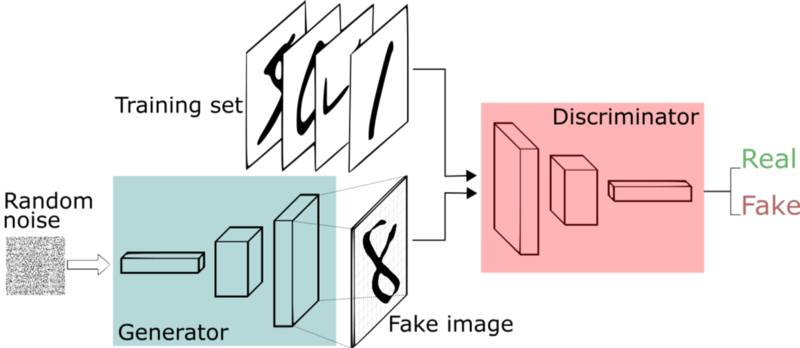
\includegraphics[width=12cm]{kapitel/2_stand_der_technik/img/GAN.png}
	\label{img:gan}
	\caption{Generative Adversarial Network (Bild von Thalles Silva \cite{img-gan})}
\end{figure}

Die beiden Netze eines GANs werden in den Generator und den Discriminator unterschieden.
Aufgabe des Generators ist die Generierung von synthetischen Daten.
Dafür wandelt er eine zufälligen Eingabe in einen möglichst realistischen Output um.
Die zufällige Eingabe dient dabei als Basis für die Ausgabedaten.
Das ist notwendig, da der Umwandlungsprozess selbst deterministisch ist, aber trotzdem eine Vielzahl an unterschiedlichen Daten generiert werden soll.
\newline

Der Output des Generators wird vom Discriminator klassifiziert.
Dafür wird er sowohl auf die generierten Daten als auch einen Bestand an echten Daten trainiert.
Sein Ziel ist es dann, die falschen Daten des Generators zu identifizieren.
Ziel des Generators hingegen ist es, den Discriminator zu täuschen und die generierten Daten als echt wirken zu lassen.
\newline

Ian Goodfellow bezeichnet den Lernprozess auch als Minimax-Spiel, bei die Ausgabe des Discriminators die zu optimierende Größe ist.
Das bedeutet, der Generator versucht die Genauigkeit des Discriminators zu verringern, während der Discriminator sie erhöhen möchte. \cite{gan-minimax} 
\newline


Für diese Arbeit werden zusätzlich Label eingeführt, um die generierten Daten beeinflussen zu können. 
Diese Art von GAN nennt sich CGAN oder Conditional GAN \cite{gan-conditional}.
Dazu erhalten der Generator und Discriminator das Datenlabel als einen weiteren Input.
So kann der Discriminator aus den echten Daten lernen, dass Daten bei bestimmten Labeln bestimmte Eigenschaften haben.
Dadurch ist dann der Generator gezwungen, diese Eigenschaften zu berücksichtigen, um den Discriminator wieder zu täuschen.

\section{Ausprägungen von GANs}
\todo[inline, shadow]{Hier DC-GAN usw. nochmal erklären, weil die Begriffe sind nicht so eindeutig!}
Die folgenden Ausprägungen von GAN Architekturen unterscheiden sich Primär in den verwendeten Layern.

\subsection{CGAN}
\todo[inline, shadow]{Formel aus dem Paper: \cite{mirza2014conditional}}
Bei einem Conditional GAN \cite{mirza2014conditional} wird neben der Latent-Dimension zusätzlich noch ein Label übergeben.
Dies geschieht sowohl beim Discriminator als auch beim Generator.
Das Label gibt eine bestimmt Klasse der Daten an und wird dann auch beim Trainingsprozess berücksichtigt.
Das bedeutet, der Discriminator bekommt bei Label X nur Daten des Labels X zum Vergleich vorgelegt.
\newline

Sobald das GAN zufriedenstellend trainiert ist, können so labelspezifische Daten generiert werden.
Das kann in der Praxis sehr günstig sein, wenn zum Beispiel das Krankheitsbild einer bestimmten Krankheit generiert werden soll.
Aber die Nutzung des Conditional Discriminators erlaubt beispielsweise die Identifizierung einer bestimmten Krankheit auf einem Bild.

\subsection{Dense-GAN}
Eine Dense-GAN nutzt sowohl für Discriminator als auch für den Generator Dense Layer beziehungsweise Fully Connected Layer.
Dense Layer bestehen aus Neuronen, die jeweils mit jeder Ausgabe der vorherigen Schicht verknüpft sind.
\newline

Vorteil dieses Architekturmodells ist seine große Flexibilität.
Mithilfe der Dense Layer und einer ausreichend großen Architektur lassen sich theoretisch alle Zusammenhänge eines Datensets lernen.
\newline

Nachteil sind die vielen zu lernenden Parameter.
Pro Schicht ergeben sich $|weights| = inputs * outputs$, was bei größeren Architekturen einen erheblichen Lernaufwand bedeutet.
Insbesondere im Vergleich zu Convolutional Layern macht dies einen enormen Unterschied.

\subsection{DC-GAN}
\todo{Belege}
Ein DC-GAN oder auch Deep Convolutional GAN besteht hauptsächlich aus Convolutional Layern.
Im Generator finden vor allem Convolutional Transposed Layer ihre Anwendung.
Convolutional Transpose Layer funktionieren wie Convolutional Layer, jedoch vergrößern sie Ausschnitte, statt sie zu komprimieren.
Im Discriminator werden Convolutional Layer genutzt, um die Datenmenge auf eine Entscheidung klein zu skalieren.
Im letzten Schritt des Discriminators existiert in der Regel ein Dense Layer, um die finale Entscheidung zu berechnen.
\newline

Vorteil dieser Architektur sind die vergleichsweise wenigen zu lernenden Parameter.
Die geringe Anzahl an Parametern sind der Tatsache geschuldet, dass es pro Ausgabe-Dimension nur einen Filter für das Convolutional Layers gibt.
Dadurch ist auch die Parameteranzahl der Convolutional Layern unabhängig von der Bildgröße.

Zusätzlich zur geringen Parameteranzahl fördern die Filter auch das Verständnis von Zusammenhängen zwischen benachbarten Pixeln.
Die Zusammenhänge werden dabei implizit durch die Architektur vorgegeben und müssen nicht erst aufwändig gelernt werden.
\newline

Die Tatsache, dass die Filter der Convolutional Layer so viel vorgeben ist jedoch auch gleichzeitig ein Nachteil der Architektur.
Sollten die Beziehungen zwischen nahen Datenpunkten nicht existieren, werden falsche Zusammenhänge impliziert, was zu schlechteren Ergebnissen führen kann.
Insgesamt ist eine solche Architektur somit nicht so flexibel wie eine Dense Architektur, aber dafür effizienter.

\section{Verfahren zur Bestimmung von Hyperparametern}
\label{chapter:verfahren-bestimmung-hyperparameter}
\todo{Quelle \cite{hyperparameters-search}}

Die Bestimmung guter Hyperparameter ist im Rahmen der Arbeit von großer Bedeutung, da verschiedene Architekturen auf ihre Effektivität und Effizienz untersucht werden sollen.
Bei gleichen Hyperparametern für verschiedene Architekturen wäre dies ein unfairer Vergleich.
\newline

Für die Suche nach optimalen Hyperparametern gibt es verschieden Verfahren, die im Folgend vorgestellt werden.
Dabei wird sich auf die Grid Search, Random Search und den Genetic Algorithm beschränkt, da diese die beliebtesten Algorithmen zur Optimierung sind \cite{hyperparameters-search-comparison-focus-genetic}.
Die Verfahren werden zusätzlich mit der manuellen Suche verglichen, um eine allgemeinere Einschätzung gewährleisten zu können.

\subsection{Manuelle Suche}
Die manuelle Suche ist das simpelste vorgestellt Verfahren.
Hierfür werden nur die Hyperparameter vor jedem Trainingsdurchlauf manuell festgelegt.
Nach einem Trainingsdurchlauf können dann die Ergebnisse analysiert, Hyperparameter angepasst und die verbesserte Version erneut trainiert werden.

%Die manuelle Suche ist vor allem bei unwichtigen Hyperparametern sinnvoll, da dort bekannte Standardwerte gesetzt werden können.
%Für eine gründliche Suche aller Hyperparameter ist die manuelle Suche allerdings viel zu aufwändig.

\subsection{Grid Search}
Bei der Grid Search handelt es sich um eine sehr traditionelle Technik, die gut mit einem Brute-Force Ansatz vergleichbar ist \cite{hyperparameters-grid-search}.
\newline

Für die Suche werden zunächst die zu untersuchenden Hyperparameter ausgewählt.
Danach erfolgt die Definition eines Suchintervalls inklusive Intervallschritten für jeden Hyperparameter.
Schließlich wird das neuronale Netzwerk für jede Kombination der Hyperparameterwerte trainiert und die Ergebnisse der einzelnen Durchläufe festgehalten.
Die Trainingsdurchläufe können dabei parallel stattfinden.
Dadurch entsteht zwar ein erhöhter Speicherbedarf, jedoch wird die Trainingszeit stark beschleunigt.

Nach dem Training ist es dann möglich, die einzelnen Ergebnisse zu vergleichen.
Dabei können dann Schemata erkannt und Kombinationen aussortiert werden.
%Es ist dann möglich die erfolgversprechendsten Netze weiter zu trainieren, oder direkt eine zufriedenstellende Kombination auszuwählen.
\newline

Insgesamt ist Grid Search sehr simpel zu implementieren, aber auch sehr ressourcenaufwändig.
Der exakte Aufwand hängt dabei stark von der Anzahl der möglichen Kombinationen der Hyperparameterwerte ab.
Da es sich bei den Kombinationen um ein ein Kreuzprodukt handelt, wächst der Aufwand mit der Anzahl an Werten sehr stark an.
Durch die Möglichkeit von Parallelisierung findet die Grid Search in der Regel bessere Parameter als die sequentielle manuelle Suche in der gleichen Zeit \cite{hyperparameters-random-search}.

\subsection{Random Search}
Die Random Search \cite{hyperparameters-random-search} funktioniert ähnlich wie die Grid Search, nur werden zufällige Werte statt einem festgelegten Werteraster erzeugt.
\newline

Die zufälligen Werte haben den Vorteil, dass es weniger Werte-Überlagerungen im Vergleich zur den Raster-Kombinationen gibt.
Deswegen kann die zufällige Suche bei gleich vielen Durchläufen ein größeres Spektrum an Ergebnissen abdecken.
Mittels \textit{Automatic Relevance Determination} \cite{automatic-relevance-determination} ist es dann möglich, den Einfluss und Wertebereich der einzelnen Hyperparameter darzustellen.
\newline

Vorteil der Random Search im Vergleich zur Grid Search ist, dass keine Hyperparameter festgelegt werden müssen.
Das erlaubt eine unvoreingenommene Herangehensweise an die Suche.
\newline

Problem der Random Search ist vor allem, dass die Räume der guten Hyperparameter (\textit{Search Space}) sehr klein sind.
Dadurch ist nicht gewährleistet, dass ein zufälliger Wert auch den Raum der optimalen Werte trifft.
Jedoch erzielen Hyperparametersuchen mittels Random Search in der Regel trotzdem (sehr) gute Ergebnisse.
Dem Grid Search Verfahren ist die Random Search allerdings nicht prinzipiell überlegen \cite{hyperparameters-random-search}.
\newline

Aufgrund ihrer Ähnlichkeit teilt sich die Random Search auch das Problem der Ressourcenintensivität mit der Grid Search.
Sobald ein sehr großes Spektrum an Hyperparametern untersucht werden soll, benötigt sie sehr viel Zeit.
Je nach zusätzlichen Optimierungen für die Wahl der Zufallswerte lässt sich die Random Search auch nicht unbedingt parallelisieren, was zu einer sehr langen Laufzeit führen kann.

\subsection{Genetic Algorithm}
\todo[inline,shadow]{mehr belegen}
Der Genetic Algorithm wandelt die Hyperparametersuche in einen evolutionären Entwicklungsprozess um.
Der Evolutionsaspekt des Algorithmus ist dabei eine Anlehnung an die natürliche Entwicklung in der Natur.
Diese Entwicklung zeichnet sich durch die Operatoren \textit{Selektion}, \textit{Kombination} und \textit{Mutation} aus, die der Algorithmus verwendet \cite{hyperparameters-genetic-algorithm}.
\newline

Für den Optimierungsprozess werden am Anfang mehrere zufällige Hyperparameterinstanzen erzeugt.
Die Instanzen werden dann trainiert und stehen im Wettbewerb um das beste Ergebnis.
Nach der Auswertung der Trainingsergebnisse werden die besten Instanzen selektiert und miteinander gekreuzt und oder mutiert.
\newline

Der Genetic Algorithm eignet sich besonders gut bei sehr vielen Hyperparametern.
Im Gegensatz zur Grid Search werden nicht immer alle Kombinationen ausprobiert, sondern nur einzelne, die sich bereits zuvor als vielversprechend herausgestellt haben.
Dadurch kann mit sehr großen Mengen an Hyperparametern umgegangen werden.
\newline

Allerdings ist der Genetic Algorithm vergleichsweise langsam, da die Evolutionsschritte sequentiell ablaufen müssen.
Erst bei einer hohen Anzahl an Hyperparametern oder einem sehr großen Suchraum ist der Genetic Algorithm effizienter als eine Grid Search \cite{hyperparameters-search-comparison-focus-genetic}.

\section{Related Work}
\label{chapter:related-work}
In diesem Kapitel werden ähnliche Werke vorgestellt, die einen Bezug zu dieser Arbeit haben.
Allerdings existieren keine Werke, die sich exakt mit dem gleichen Thema beschäftigen.
Jedoch gibt es trotzdem Gemeinsamkeiten zu anderen Arbeiten, an denen sich in diesem Projekt orientiert werden kann.
Das ist insbesondere der Fall, wenn die Daten ähnlich sind.
Ähnlichkeit bedeutet in dem Fall eine ähnliche Bildgröße oder Farbe.

\subsection{CGAN - MNIST}
Das Paper \textit{Conditional Generative Adversarial Nets} \cite{mirza2014conditional} befasst sich allgemein mit der Erweiterung von GANs durch Conditions. \todo{anderes Wort als Conditions?}
Die vorgestellten CGANs werden hierfür auf die Datensets MNIST und Flickr trainiert.
Ziel ist dabei nicht, eine optimale Netzarchitektur oder Ergebnisse zu erzielen.
Stattdessen stellt die Arbeit einen Machbarkeitsbeweis für CGANs im Allgemeinen dar.
\newline

Auf dem Paper aufbauend existiert ein Tutorial Notebook \cite{cgan-tutorial-notebook}, noch einmal explizit für das MNIST Datenset.
Das ist zwar der gleiche Datensatz, der auch im Paper genutzt wird, jedoch wird dort die genaue Netzarchitektur nur grob beschrieben.
Das Notebook hingegen enthält sogar Codebeispiele in Tensorflow, die eine Beispielimplementation bilden.
\newline

Die Architekturen von sowohl dem Generator, als auch vom Discriminator bestehen ausschließlich aus Dense Layern.
Auf jede Dense Layer Schicht wird dann zusätzlich LeakyReLU und BatchNormalization angewendet.
Als Eingabe erhält der Generator zum einen die Latent Dimension mit 100 zufälligen Zahlen und als Condition eine one-hot Vektor mit 10 Zahlen, die den MNIST-Zahlen-Klassen entsprechen.
Nach 100 Epochen Training erreicht diese Architektur die folgenden Ergebnisse \todo{bei genug Seiten (inklusive Bild) raus nehmen, weil eigentlich ist das irrelevant}:

\begin{figure}[H]
	\centering
	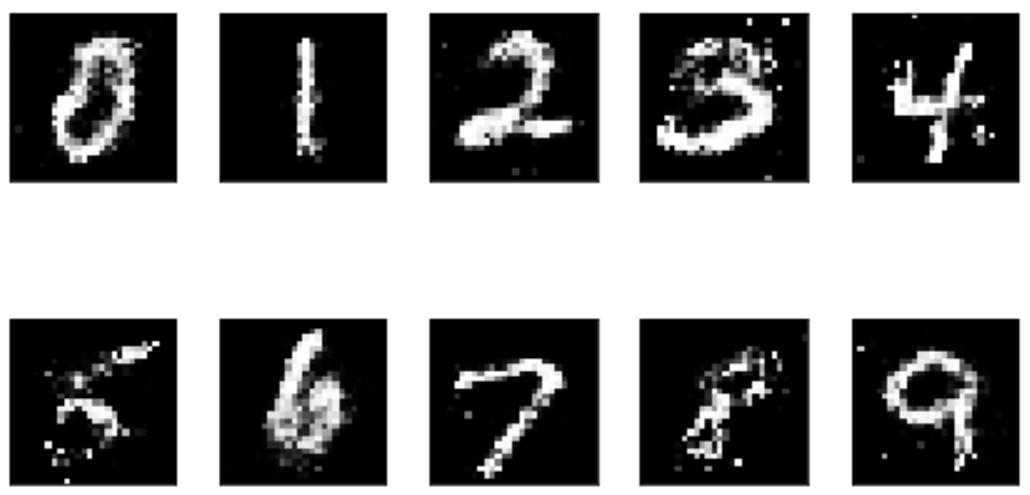
\includegraphics[width=7cm]{kapitel/2_stand_der_technik/img/cgan-notebook-ergebnisse.png}
	\caption{Ergebnisse Notebook \cite{cgan-tutorial-notebook}) }
\end{figure}

\subsection{LightCovidNet}
Das LightCovidNet \cite{inspiration-dc-gan-med} erlaubt die Erkennung von Krankheitsfällen in Lungen Röntgenscans.
Bei den Krankheitsbildern handelt es sich um COVID-19 und virale Lungenentzündungen.
Das Netz wurde dafür zum Teil auf synthetische COVID-19 Bilder trainiert, um einem Missverhältnis an Bildern für die Krankheiten in den Trainingsdaten entgegenzuwirken.
Das zur Generierung verwendete GAN erlaubt die Erzeugung von allen Krankheitstypen und auch Bildern von gesunden Lungen, wobei für die Arbeit nur die Generierung von COVID-19 Bildern von Interesse war.
\newline

Das dadurch entstandene GAN ist auch für diese Arbeit interessant, da es in der Lage ist, komplexe Formen mithilfe von relativ weniger Parameter zu generieren.
Die Parameteranzahl ist so gering, da in der Architektur hauptsächlich Convolutional(-Transpose) statt Dense-Layern eingesetzt werden.

\begin{figure}[H]
	\centering
	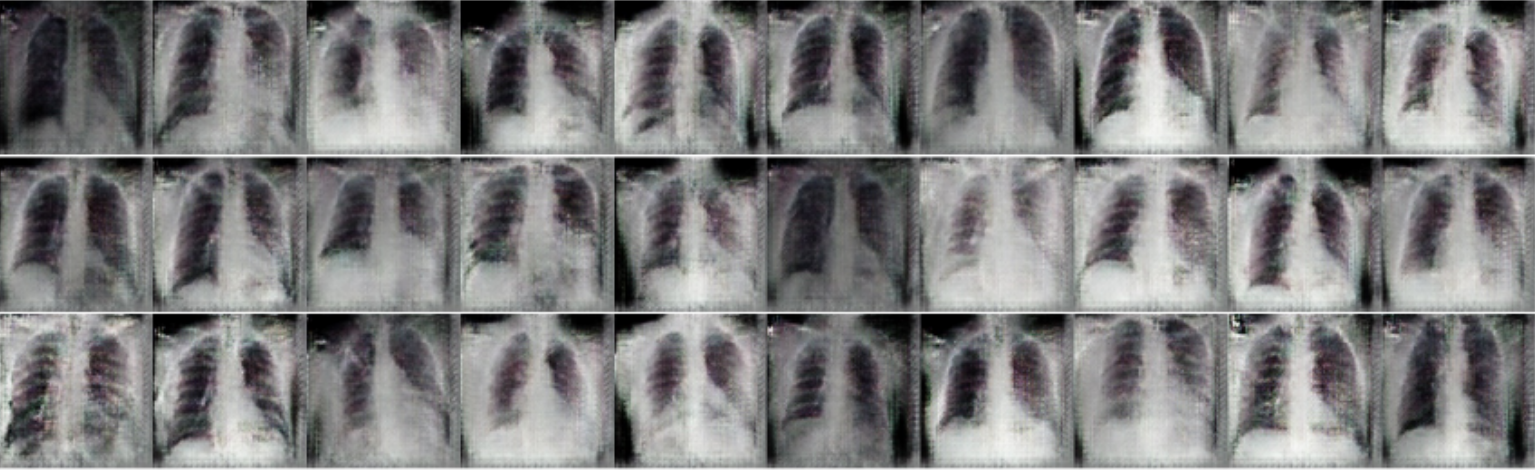
\includegraphics[width=9cm]{kapitel/2_stand_der_technik/img/light-covid-net-ergebnisse.png}
	\caption{Ergebnisse GAN aus LightCovidNet \cite{inspiration-dc-gan-med}}
\end{figure}


\begin{comment}
	
\paragraph{Links}
\begin{itemize}
	\item Inception Score zum Rating von erzeugten Bildern (Salimans et al. 2016)
	\item Frechet Inception Distance (Heusel et al. 2017)
	\item stackoverflow \url{https://stackoverflow.com/questions/46386948/adjusting-gan-hyperparameters}
	\item \url{https://openreview.net/pdf?id=rkGG6s0qKQ}
	\item \url{https://arxiv.org/pdf/1511.06434.pdf%C3%AF%C2%BC%E2%80%B0}
	\item Forget the Learning Rate, Decay Loss \url{https://arxiv.org/ftp/arxiv/papers/1905/1905.00094.pdf}
	\item beste learningRate/Dropout/BatchSize/NumberOfNeuronsInDenseLayer mit evolutionären neuronalen netz für mnist 
	\item zum orientieren ?? \cite{gan-conditional}
\end{itemize}


\end{comment}